\chapter{Escalamiento}

Scrum es aconsejable para ser óptimo en equipos chicos y proyectos pequeños, con agrupación de personas de múltiples disciplinas en un solo equipo para maximizar el ancho de banda de las comunicaciones, la visibilidad y la confianza. Esto sucede porque cuando los equipos son grandes aumenta el acoplamiento de individuaos complejizando las comunicaciones y dificultando la coordinación y el buen desarrollo de las reuniones Scrum. Además se desprende del principio o Ley de Brooks , que cuando se agregan personas a un proyecto o equipo aumentan los canales de comunicación pudiendo generar sobrecarga de comunicación. Por este motivo y desde un punto de vista purista, cuando se quiere implementar Scrum en proyectos grandes que requieren muchas personas, en su forma ortodoxa, no es recomendable. Pero se han encontrado maneras organizativas para aplicar Scrum en estos casos. Una forma es el uso de equipos Scrum de características, equipos Scrum de componentes y el uso de "Scrum de Scrum".

\section{Equipos de características}

Abordar el problema de proyectos grandes con "Equipos Scrum de características" consiste en la conformación de equipos totalmente multi-funcionales, capases de operar en todos los niveles de la arquitectura del producto con el fin de ofrecer las características centradas en el cliente. O sea que cada equipos trabaja sobre determinadas características de producto (Features) o PBIs desarrollando todos los niveles del sistema a desarrollar. En este sentidos, los equipos son homogéneos entre si pero eterogéneos internamente, con integrantes de habilidades diversas y características profesionales multidisciplinares. Para lograr esto se debe conformar una organización de aprendizaje donde los equipos practican el aprendizaje continuo, donde aprenden para abarcar los componentes arquitectónicos. 

\begin{figure}[h]
  \centering
  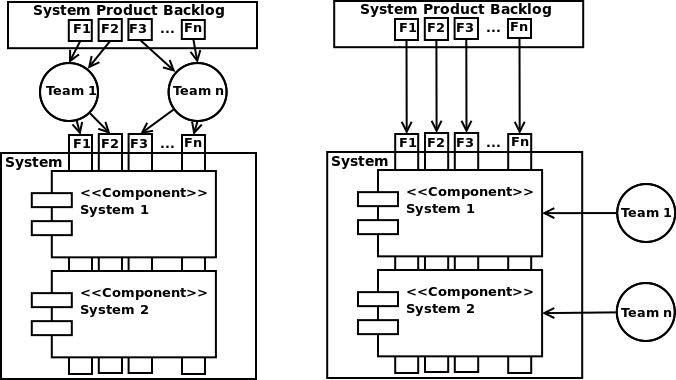
\includegraphics[scale=0.4]{ScrumTeamsByFeaturesAndByComponents}
  \caption{Equipos de Características (izq.) y Equipos de Componentes (derecha)}
  \centering
  \label{fig:ScrumTeamsByFeaturesAndByComponents} %\ref{fig:ScrumTeamsByFeaturesAndByComponents}
\end{figure}

En esta arquitectura de organización es necesario coordinar el trabajo de los diferentes equipos. Los Scrum Master deben reunirse con regularidad, promoviendo la transformación a travez de una lista visible de los impedimentos de organización. Los Scrum Master, además deberan estar familiarizados con biografía relacionada a este proble de escalabilidad como "Scaling Lean and Agile Development" \cite{Larman-Vodde-2008}.

\section{Equipos de componentes}

\section{Scrum de Scrum}

Scrum de Scrum es una forma de organización y técnica para escalar Scrum a grupos grandes de personas. Consiste en distinguir un integrante con el rol de Embajador, denominado "Ambassador", por cada Equipo Scrum \cite{Stefanini-2013}. El Embajador será quien participará en reuniones Daily con Embajadores de otros equipos. A esta reunión de Embajadores se la llama "Scrum de Scrum". Habitualmente se usa que el rol de Embajador lo desempeñe el Scrum Master, pero puede ser desempeñado por otro integrante del Equipo de Desarrollo. La reunión “Scrum de Scrum” se comporta como una Daily donde los Embajadores reportan la cituación de su equipo y sus impedimentos.
